\chapter{Security Aspects}
\label{chap:5}
%
As autonomous vehicles are getting closer to reality as private and public mean of transportation, it is natural to be interested in safety and security which these new technologies are promising. A number of security vulnerabilities and concerns related to autonomous vehicles can become a potentially deadly weapon in the future \cite{selfDrivingCarSec}. But greater concern than terrorism attacks on autonomous vehicles are the risk of controls systems being hacked in and taking control of a driving or other essential systems and in this way to put into a dangerous situation driver or passengers of the car. 
This can sound too non-realistic, but \textit{white hat hackers} for years already have been showing security issues related to connected cars, demonstrating how easy is to take control and do harm over a lot of various systems even in non-automated vehicles. One of Chinese security company demonstrated that it is very easy to spoof sensors of a vehicle, causing them to sense "ghost" objects or fail to detect a real object at all \cite{ChinaAttack}.
Here natural question can arise, so what makes autonomous vehicles so vulnerable against malicious attacks as compared with non- or only partial autonomous cars? Authors of \cite{sec} suggesting two main reasons:
\begin{enumerate}
	\item \textbf{The increased interaction between autonomous cars and environment.} At the moment the most communications between vehicles on the road occurs via \glspl{VANET}. This type of communication allows sharing fast changing surrounding information with vehicles which are nearby communicating vehicle. This allows for other cars/drivers in the cars to be aware of what is the road situation nearby them \cite{carspeak}. Since technologies are improving and fully autonomous cars will be on the roads in the very near future, \gls{V2I} and \gls{V2IoT} communication will be more common on the roads. Due to connectivity in one network, only one "infected" vehicle can compromise the entire network if the network is not properly secured.
	\item \textbf{The increased interaction between components of the system inside, so-called intra vehicular communication.} Autonomous cars have a lot of different \glspl{ECU} which are connected with each other using \gls{CAN} bus. One of the biggest advantages of using \gls{CAN} bus is that it is like a central unit into which a lot of different modules can be added or removed without changing the wiring architecture in the car. \gls{CAN} has three main parts:  \textbf{Data link layer}, which is responsible for data transferring. \textbf{High speed} physical layer and \textbf{Low speed} physical layer which is also responsible for fault toleration. In most cases, the most important control units (which has a direct impact on safety, e.g. brake or engine control module) are connected to high speed layer and others, not so security sensitive are connected to low speed layer. Not so common situation, but it is possible to have a "gateway bridge" which opens the route for selected packages from low to high (or vice versa) layers. So it is a possibility that that malicious packets are connected to the \gls{CAN} bus using low speed layer and without any further checking or suspicion it can be transferred into high speed layer causing to serious consequences. Control architecture in autonomous vehicles is working in this way what all nodes get packages from \gls{CAN}. Any malicious component which is connected to the internal vehicle network can snoop all communications or it can infect all other elements. In order to protect the network, every path for package moving should be protected to ensure the vehicle security. Unfortunately, it is impossible to predict all possible attacks and to foresee all vulnerable places, because there always be new strategies which will threaten the security of autonomous cars. "The development and improvement of one will always counteract and necessitate the development of another" \cite{sec}. \\	
	Another cause of \gls{CAN} vulnerabilities is that all \gls{CAN} packages are not authenticated before using them for communication within the system. Any element of a network can send infected element further if former did not do any validation of the package before accepting it \cite{secanalysis}.
	One way to protect network infrastructure is to use packet-level authentication method. This method allows authenticating a package without having trust association of the package sender \cite{pla}.
\end{enumerate}

\section{General Overview. Attack Taxonomy}

This section will introduce the potential threats, vulnerabilities
and attacks of autonomous vehicles can face. For categorization of attacks, we use way proposed in \cite{sec}. Each attack is classified based on: \textbf{Type} (or source) of the attacker, \textbf{Attack vector} (path and method which was taken to get access to the vulnerable place), \textbf{Target}, \textbf{Reason/objective/motive} of the attack and \textbf{Potential outcome}.

Figure~\ref{fig:AttackTaxonomy} summaries attack taxonomy which will be described in this section.

\begin{figure}[h]
	\centering  	
	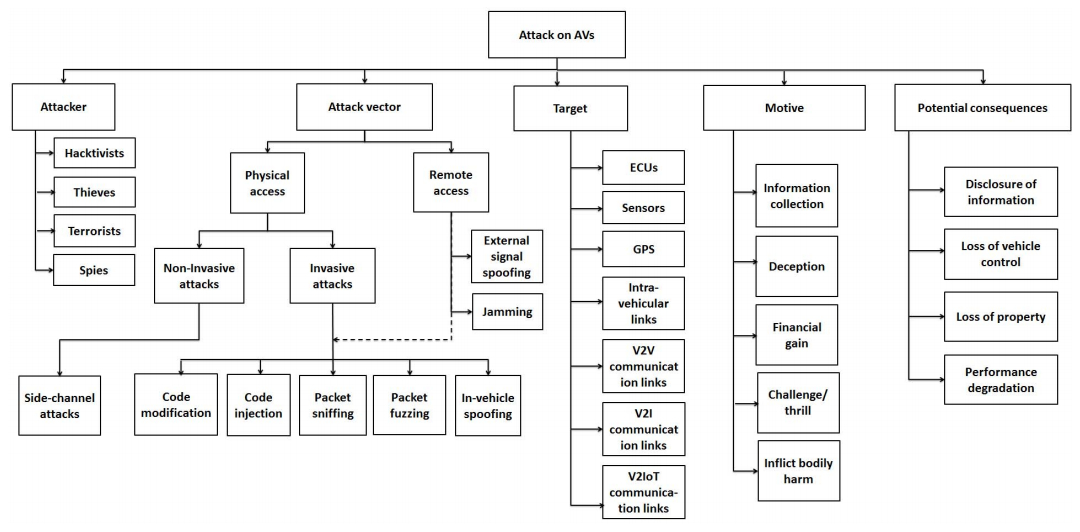
\includegraphics[width=17cm]{img/6.jpg}
	\caption{Autonomous Vehicle Attack Taxonomy, proposed in \cite{sec}}
	\label{fig:AttackTaxonomy}    
\end{figure}

\subsection{Attacker}

It is a source of the attack. Usually, when system face an attack it tries to mitigate that immediately. One of the steps of mitigation should be an identification of attack source. Having this information it is possible not only to prevent future attacks, but also understand why the attack was implemented in the first place.
	
\subsection{Attack Vector}
It is a way how the attacker got access to the system he is targeting. It is also an enabler for an adversary to exploit the targeted system. Attack vectors can briefly be categorized to \textit{physical} and \textit{remote} access.

\subsubsection{Physical Access}
These attacks are classified into invasive and non-invasive attacks.

\begin{enumerate}
	\item \textbf{Non-invasive Attacks}: these attacks have no physical contact with the car, usually, embedded devices are used for attack implementation. However, being relatively close to the targeted vehicle is necessary in order attack to work. Example for non-invasive attacks, can be \textit{side-channel attacks}. These kind of attacks usually ends with leakage of useful information about transmitted data or about internal working paths within the system. The most common defense against this attack is employing asynchronous information processing units or/and "shielding"	mechanisms.
	
	\item \textbf{Invasive Attacks}: the main difference as compared to non-invasive attacks is that invasive attacks include a physical connection to the targeted system. The result of this attack can be the network security and \glspl{ECU} can be compromised. Potential way how adversaries can connect to the car and gain access to its \glspl{ECU} is \gls{OBD-II} port which is usually used for car diagnostic. Another way to reach a car is wireless remote access, this is possible when an autonomous car is connected to the critical infrastructure, e.g. someone in the car connects a smartphone for entertainment reasons, and in this way, all internal system can be exposed to external people or networks. There are different types of invasive attacks which are discussed below.
	\begin{enumerate}
		\item \textit{Code Modification}:this attack may happen when attacker change the code with malicious modifications in order to compromise the system. This may be achieved by connecting \gls{OBD-II} scanner to the car. As mentioned before this is a tool for vehicle diagnostic, meaning that it is widely available for anyone who wants to buy it. This attack can be avoided by ensuring that all connection to the car is password protected, which enable only certified people to connect and modify codes of the car.
		\item \textit{Code Injection}: this is a very similar attack to the previous one. In this case, after connecting to the car, the attacker can inject new (most likely malicious) code instead of modifying the old one. Code injections can be made not only by an attacker, the owner of the vehicle or person who is checking a car can also inject a new code, hoping to improve the performance of a vehicle. When injected codes are non-compliant with car's components or when new codes are not proved by authorities, problems can appear. One of the ways to avoid code injections is a usage of the intrusion detection system or/and usage of privileged access, which allows only authorized people to connect to the car, owner excluded.
		\item \textit{Packet Sniffing}: also known as package analyzing. For this attack computer program or hardware, called sniffer (or analyzer) is used. A packet sniffer can see details between any communication node. The tool is very useful when network related problems need to be diagnosed. But the tool can be used for malicious purposes as well: an attacker can use sniffers for collecting unprotected information, for eavesdropping or capturing packages for following replay attack. Defenses for this attack can be various encryption techniques for confidentiality in packages protection, as well as usage of real-time packages send/received update messages.
		\item \textit{Packet Fuzzing}: this technique usually is used during security testing procedures, when invalid data is sent to the system/element, expecting to get receive some error or fault conditions, which allows exploiting weak places in the system and security loopholes. While testing the system, fuzzing helps to detect problems and utilize them in a further stage. When this technique is used by adversaries, the received information is used to get into the system and do any possible harm. Protection against fuzzing is to fix all errors and security loopholes immediately after its exposure. 
		\item \textit{In-Vehicle Spoofing}: is a situation in which an attacker, using some software tools, pretending to be another person by falsifying data. In this way, adversary gains an illegitimate advantage. In order to attack be successful adversary needs to overcome security mechanisms (if exists) to replace original elements with spoofing devices. Usual defenses for this is into autonomous car network include reply attack resistance techniques and fingerprinting module to be able to differentiate between original and current module in the vehicle system \cite{attacTax1}.
	\end{enumerate}
\end{enumerate}

\subsubsection{Remote Access}
Since wireless connection to external sensors, such as cameras, \gls{LiDAR}, \gls{RaDAR}, \gls{GPS} are getting more and more popular and useful while driving, attackers can also use remote access as method to attack systems of autonomous vehicles. 

\begin{enumerate}
	\item \textbf{External Signal Spoofing}: one example for this type of attack is \gls{GPS} spoofing. This attack is possible because \gls{GPS} using a wireless connection. During the attack \gls{GPS} receiver is deceived by sending the wrong signal to \gls{GPS} from another device. The incorrect signal may be similar to real \gls{GPS} signal or can be captured before and replayed at a certain time. An attacker can trick \gls{GPS} receiver to accept and recognize only fake signal by gradually increasing power strength of the wrong signal until it eventually replaces the original signal. As soon as the attacker gains control of \gls{GPS} device in an autonomous car, he can send false \gls{GPS} information and lead car in the wrong direction and destination. This attack was not tested on autonomous cars, but it was successfully tested on \gls{GPS} devices in \gls{UAV} and yachts \cite{Spoof2, IIIspoof}. \\
	\gls{GPS} devices are not the only target in autonomous cars. Vehicles contain numerous sensors, which can be attacked with spoofing. One of these devices could be visual sensors like cameras, \glspl{LiDAR}. Similar to the previously described attack was made on \gls{LiDAR} sensor in \cite{AttacksOnSensors}. Sending fake signals to the device in a range between $20$ and $250$ meters from a car (sensor) a lot of non-existing obstacles can be detected as well as existing obstacles on the road can be missed. 
	The way to protect the system against spoofing attacks is to ensure more security, not to accept any signals and information without checking the authenticity and integrity of a signal sending device. To ensure that correct information is coming to \gls{LiDAR} additional information sources can be used and perform information checking between two different devices. If this cross-checks matches and succeeds information is more likely to be correct than in a case when information is not matching between different sources.
	\item \textbf{Jamming}: these attacks are against wireless or external sensors for vision and due to that, the authorized communication might be destroyed. The most sensitive devices for jamming attacks are \gls{LiDAR}, \gls{RaDAR}, various cameras. Jamming devices can block sensors for receiving correct data. Authors of \cite{AttacksOnSensors} used jamming to blind cameras of autonomous vehicles to hide objects on the road and make map "cleaner" as it is. There are ways to protect sensors against this attack using removable near infrared-cut filter to the camera, however, this method is working only in the day time. Another measure is photo-chromic cameras' lenses, which can filter out specific types of light.
\end{enumerate} 

\subsection{Attack Target}

The target component of the car is usually depends on motive/object of attack and attacker’s intention. If the attacker wants to track a path which car is moving, the target element can very likely be camera and/or \gls{RaDAR} or \gls{LiDAR} , since they are vision elements of the car and having information from these sensors it is easy to see and follow the path, car took. If attacker targeting traffic optimization and/or passengers safety, as a target \gls{VANET} can be used, ect.

\subsection{Attack Motive}

Various motives for attacks are possible, better we understand it, it is more likely to protect all control systems and ensure safe driving. One of possible reasons for attacking can be deception - this is a spreading a false information, hoping to effect behavior of other, this attack may lead to hazardous situations on the traffic/roads. Another motive can be economical - to get a financial gain. One more reason can be, due the any reasons, cause severe to passengers of the car, etc.

\subsection{(Potential) Consequences}

Various consensuses are possible if any of these attacks against autonomous vehicles will be successful, such as some (important) control functions might to fail or be sabotaged, data leakage (e.g. vehicle movement information) is very possible outcome \cite{sec, secsec}. The "health" of the system is very likely will be affected after successful attacks, which can lead to passengers of the car health issues. \\

Another important problem which must to me mentioned while talking about security issues on autonomous cars and is not mentioned in attack taxonomy yet is \textbf{privacy}. An attacker can arrange an attack where he follows car movement, times and makes a very detailed profile about car owner and with this information can do various things: from robbing the house of the victim while he is not at home, to selling this information to someone else, combine different attacks to do the biggest damage attacker want (or is able) to arrange.

\section{General Overview. Defense against Attacks Taxonomy}

As mentioned earlier it is very hard to predict what is going to happen to prevent yourself against attacks. However, with current knowledge about system and known potential vulnerabilities, it is possible to make some kind of predictions and develop network architectures and working protocols which are not so vulnerable. Various literature surveys propose the main $4$ types of defenses for autonomous vehicles: \textbf{Preventive}, \textbf{Passive}, \textbf{Active} and \textbf{Collaborative} defenses \cite{secsec}. \\
This classification and different ways of protection ensure that the system is secure and resilient for different attacks. Figure~\ref{fig:DefenseTaxonomy} summaries defense against attacks taxonomy described in this section.

\begin{figure}[h]
	\centering  	
	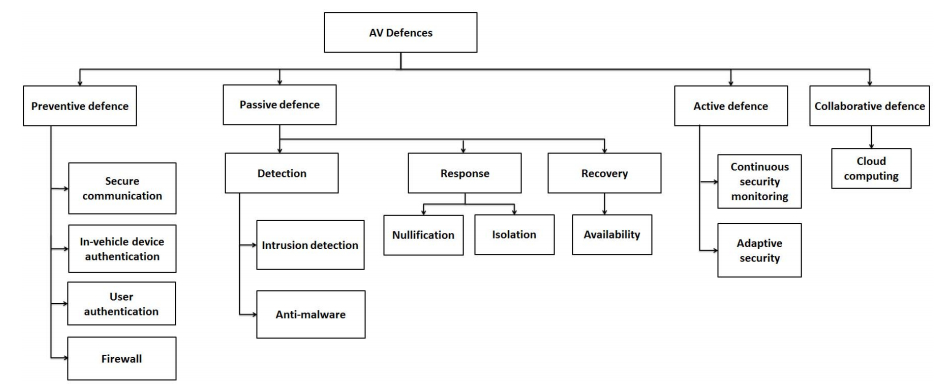
\includegraphics[width=17cm]{img/7.jpg}
	\caption{Autonomous Vehicle Defense Taxonomy, proposed in \cite{sec}}
	\label{fig:DefenseTaxonomy}    
\end{figure}

\subsection{Preventive Defense}

This type of defense mechanisms mainly focuses on protecting a system from attack before it starts or finishes with success. Preventive defense is mainly focusing on normal working conditions and not during the attack and does not solve any issues with "after attack" scenarios.	
\begin{enumerate}
	\item \textbf{Secure Communication}: for secure communication data encryption is basic and crucial. Using encryption content and confidentiality of messages are assured. Encryption scheme can also help with the identification of sender/received of sent data. To know the integrity and authentication of another side of communication is very important for secure communication.
	\item \textbf{In-Vehicle Device Authentication}: controllers used in the car can be completely trusted if they have a manufacturer certificate which gives information such us controller identifier, public key, information about authorized carryout, etc. If information, provided in certificate matches with information which car itself contains, then authentication process is successful and car safely can use all information coming from that particular controller.  
	\item \textbf{User Authentication}: sometimes, in order to have more protection, user authentication is used. To make sure that the right person has access to the car (e.g. doors opening, starting the car, etc.) additional biometric information can be used. 
	\item \textbf{Firewall}: it is an additional tool, which always can be used. Firewalls check all incoming and outgoing data traffic based on rules which user/authenticated people can define. Firewalls also can be very helpful in communication with a trusted and not-trusted environment: this is very important while communicating with different objects in vehicles' networks.
\end{enumerate}
		
\subsection{Active Defense}
This is one of the advanced and determined defense techniques. Different approached described below.	

\begin{enumerate}
	\item \textbf{Continuous Security Monitoring}: autonomous vehicles belong to critical infrastructure and it is essential that security of these systems should not be compromised. It must have (near) real-time solutions for checking and/or restoring healthy driving conditions in the car. Non-stop and continuous monitoring and "snapshots" of all running systems are required to be available for security checking at any time. 
	\item \textbf{Adaptive Security}: Nowadays the most critical systems are fast changing or refer to infrastructure with a fast pace, it is necessary to model and use defense mechanisms which are dynamic. So-called adaptive reconfigurations for target can be used for ensuring better control and balance during attack. In order to prepare it self for future attacks defense mechanisms should be able to analyze past and current attacks and use self learning mechanisms to predict what may happen in the future and adapt defense mechanisms for new forms of attack in the future.
\end{enumerate}	
		
\subsection{Passive Defense}
Passive defense measures are taken to minimize damage caused by an attacker without having the intention of taking initiative. A passive defense can be an additional level of protection (not the main one). As compared to active defense, the passive defense does not require any analysis from human.

\begin{enumerate}
	\item \textbf{Attack Detection}:
	\begin{enumerate}
		\item \textit{Intrusion Detection}: To detect physical threats to the car is much easier than to see attacks against system operations. However, there are various models for \gls{IDS} which can be used for autonomous vehicles. Authors of \cite{intrution} proposed and tested \gls{IDS} models using various computational simulation scenarios.  
		\item \textit{Anti-Malware}: these systems need to be able to protect from harmful attempts to penetrate into the main system. 
	\end{enumerate}
	\item \textbf{Attack Response}:
	\begin{enumerate}
		\item \textit{Nullification}: when an attack is recognized by system nullification can be used. This defense mechanism can neutralize an attack using cyber/electronic capabilities, e.g. \gls{GPS} signal anti-jamming technologies \cite{sec}. 
		\item \textit{Isolation}: it helps vehicles to isolate themselves from other cars during an attack. Self-isolation also prevents \glspl{ECU} re-programming while the car is running. When a car is attacked ideally it not only should isolate itself but also inform vehicles around about attack in order other cars could take some actions to defend itself against attack \cite{sec}.
	\end{enumerate}
	\item \textbf{Attack Recovery}:
	\begin{enumerate}
		\item \textit{Availability}: this feature one of the most important in all types of systems. In the context of autonomous cars, availability is very important when talking about safety inside and outside of the vehicle. In order to ensure safety and have good fault toleration within the system in autonomous cars and to ensure quick recovery after attacks, availability must be ensured in the system.
	\end{enumerate}
\end{enumerate}	

This section provided a brief summary of vulnerabilities, attacks and defense mechanism in term of security of autonomous vehicles. One of the most important things considering security is don't to stop looking for potential vulnerabilities and ways to protect the car and all network in case of attack and/or to recover as fast as possible if an attack happened. Regardless of the effectiveness of current methods, it is necessary to think about new defense mechanisms for real-time operations of the vehicle. 	

\section{Attacks Related To Intention and Movement Prediction Making}

\cite{AttacksOnSensors} proposed the scheme from three phases which described all flow in autonomous cars: Sence, Understand and Act. The first phase contains all sensors and raw data collected from them, the raw data is proceeded and represented in the second phase and finally, having all information, in the third phase decision and action can take a place. All these phases are equally important, however, all this algorithm cannot fully functioning with poor (or fake) sensors data. \\
Our proposed algorithm as observation uses only position information, due to that attacks on \gls{GPS} are presented. To improve prediction making process data from another sensor might be included in the algorithm. For environment perception, camera and \gls{LiDAR} are one of the most important sensors in the car. Further in this section will be discussed the most common and dangerous security attacks: visual sensors (on camera and \gls{LiDAR}) attacks and common privacy issues.

\subsection{Attacks on \gls{GPS}}

\gls{GPS} receives the signal from satellites collection which flies in Earth orbit. The data signal from satellites contains the payload of time-stamp, the location of the satellite. Speed of radio waves are close to the speed of light clients (cars) use the time-stamp to measure the distance of the satellite. After all data alterations signal shows latitudinal and longitudinal coordinates, giving a precise location of the object as compared to satellites. \\
At the moment attacks on \gls{GPS} is not a concern - they explored more in the laboratories at Universities rather than by criminals. However, there is a possibility to arrange attacks against \gls{GPS} and this is only a matter of time when attacks against \gls{GPS} will become a real life problem. To attack \gls{GPS} two main attacks exist: jamming and spoofing. Signal Jamming is a noise passing over the \gls{GPS} frequency a band which results as in a Denial-of-Service for the user. While signal spoofing is false data transaction to \gls{GPS}.

\subsubsection{\gls{GPS} Jamming and Spoofing}

\cite{IIIspoof} describes a spoofing attack on \gls{GPS} in a yacht. Attack was arranged strictly on academic purposes, however, it shows that it is very easy to spoof \gls{GPS}. As mentioned before, \gls{GPS} signals are received from satellites. However, researchers in the University of Texas showed that it is possible to used spoofing device and create a fake \gls{GPS} signal on Earth.  "Attackers" were sitting inside the targeted object (yacht) and started to spoof fake \gls{GPS} signal which was a bit stronger than the real \gls{GPS} signal, coming from the satellite, using their spoofing device (which is easy to buy online). The attack started when navigation system of yacht caught a fake signal. "Attackers" changed fake signal only a few degrees, but that made all systems in the yacht to think that it is not in its course (however it was). In these situations, captain, just adjust course according to \gls{GPS} readings to be on the right course. What in reality means that yacht is few degrees out of its real trajectory. Few degrees can look not too many and nothing can happen, but these alterations can cause a lot of accidents since location precision of any means of transportation is a very important variable. In the end, by changing \gls{GPS} readings the destination of the trip can end in a completely different direction than expected.\\
However, \gls{GPS} spoofing cannot take control of the driver. It just shows the wrong location to go. The driver is the one who physically modifies the path, trusting readings from \gls{GPS}.
\subparagraph{What is the difference between \gls{GPS} spoofing and jamming?} \gls{GPS} spoofing can trick the navigation system with false data, whereas jamming can disable the \gls{GPS} system entirely. An attacker can jam any noise signal with the same frequency as \gls{GPS} signal is and at the end, \gls{GPS} device cannot differentiate which signal is real, which is not, since it got a mix of everything. In this case, \gls{GPS} system is not usable at that moment. \\
To protect the system from jamming is possible by using anti-jamming devices or nullification, which was described before. To avoid spoofing attacks it is useful to authenticate the sender of the signal since now majority of \gls{GPS} systems blindly believe that \gls{GPS} signals come from satellites and do not do any sender checking. \\ \\

As mentioned before, in this thesis we are not using any data from sensors, but to improve prediction making in a real life it is very beneficial to use additional information with the position. Due to this reason more serious attacks on visual sensors, which are the most important sensors in environment perceptions, are described. 

\subsection{Visual Sensors Attacks}
 
 In reality, autonomous cars are equipped with various sensors which measure different physical properties (sound, light, distance, radio frequency, etc.), \gls{GPS}, \gls{LiDAR}, \gls{RaDAR} systems and of course maps. To ensure sensors' resilience against various attacks is one of the main challenges. And yes, any of possible attacks against sensors can cause a decision, which can end up as an accident and in the worst case can lead to fatalities. E.g. attacks on camera can cause misunderstanding of traffic signs, leading to unsafe driving conditions with additional danger to passengers in the car and/or other road participants. \gls{LiDAR} can be fooled and observe non-existing obstacle on the road and start braking, or \gls{LiDAR} can be triggered to not notice real obstacle and go directly to it. These are only a few scenarios, but all of them can make a huge impact on traffic and its' participants \cite{AttackModel}. \\

\subsubsection{Attacks on \gls{LiDAR}}

For proper car guidance, which ensures safety on the road proper visualisation on an object on and around the road is necessary. To have good quality data with image-based sensors good weather conditions is required (typically they cannot give proper geometry information under poor weather conditions, e.g. when is raining or when it is not enough light). Laser technologies here had a lot of advantages and \gls{LiDAR} was introduced. \gls{LiDAR} working principle is based on laser scanning, and it can accurately capture all types of geometry on the road and to detect a very wide range of objects. However, a very detailed grouping of objects is still a hard task for \gls{LiDAR}. Recognition of traffic signs or lanes on the road is still cameras' task. \\
The brief working principal of \gls{LiDAR} is to notice objects which are giving a reflection of a signal sent by \gls{LiDAR}. If a sent signal does not come back to the device (it can happen because of transparency of the object, absorption, range limit, when in short range there is no object, etc.), \gls{LiDAR} thinks that there is no obstacle on the road. As \gls{LiDAR} performs a very important role in environment perception for autonomous cars and uses simple methods for object noticing, such as light pulses, it is one of the most obvious targets on the autonomous cars. The easiest way to attack \gls{LiDAR} is to create "noise" and generate (or hide) objects. This section will provide a description on already existing and tested replay and spoofing \cite{AttacksOnSensors} attacks on \gls{LiDAR}

\paragraph{Signal Relaying Attacks}

Relaying the signal is an expansion of replay attack, which goal is to relay on the signal which was sent before the attack from another position (signal sent from \gls{LiDAR} is recorded and then (repeatedly) sent from a different location). This allows creating fake echoes and due to that obstacles may appear closer/further than they truly are. \\
To perform an attack, only two transceivers, one with a photodetector, sensitive to wavelength \gls{LiDAR} is operating on and one with the laser are necessary. The output of transceiver with photodetector is a voltage signal, which corresponds to the signal intensity which was sent from \gls{LiDAR} (to be able to see the signal, oscilloscope needs to be connected to the transceiver, but it is not necessary for performing an attack). The output of the first transceiver is sent to another one transceiver (which has a laser in it) to emit a pulse in as its output. \\
In \cite{AttacksOnSensors} experiments made when transceivers were in the one-meter distance from each other and in front of \gls{LiDAR}. But this position is not only one which must be used for making this attack work: it can work very well when transmitters are behind the \gls{LiDAR} with a bigger distance between each other. A relay attack on \gls{LiDAR} is most likely to be performed from the roadside, where an attacker can easily receive signals sent by \gls{LiDAR} on a car, to record them and relay them again from the different location. \\
Results of an attack, which were noticed by performing it was that before an attack \gls{LiDAR} only noticed objects detected in short distance (around $1$ meter), during the attack range of noticing objects had grown to $20$-$50$ meters - during the attack, it was noticed that \gls{LiDAR} emits not encoded pulses, and signals can be recorded, replayed and relayed to create fake echoes. Due to this movement planning and decision making can be affected, together making an impact on people and traffic safety.\\
Note, that to perform the relay attack is relatively easy and cheap, due to that it is widely used for attacking cars in general, not only for attacks on \gls{LiDAR}.

\paragraph{Signal Spoofing Attacks}

While signal relay attack can create echoes, this paragraph will show that it is easy to create fake objects using signal spoofing attacks on \gls{LiDAR} using the original signal released by \gls{LiDAR} to "replay" objects on the road and control their location.
A signal, sent from \gls{LiDAR}, travels approximately 200 meters back and forth in about $1.3$ $\mu$s. Meaning that \gls{LiDAR} should listen at least this period for incoming sent signal reflections (depending on \gls{LiDAR} type time for a signal travelling might vary a little bit). In order to make attack successfull, the fake signal must arrive to \gls{LiDAR} in this small time window, if the signal will come back to \gls{LiDAR} after this time, it won't be noticeable, that's why attacker needs to know when to release fake signal. Working principle of \gls{LiDAR} is that longer time it takes for a signal to come back, the further object is, due to that the attacker can "control" location of obstacle by delaying the original \gls{LiDAR} signal before relaying it. \cite{AttacksOnSensors} demonstrates an attack, where \gls{LiDAR} receives the fake signal after the first echo of the original signal is received. This allows tricking \gls{LiDAR} to think that obstacle is further away since the signal traveled back longer. In order to make the attack work attacker needs to have a transceiver and two pulse generators (they are needed to generate a fake signal, which is sent back to \gls{LiDAR}). The output of transceiver is connected with the input of one pulse generator (this generator delays its output). The output of this pulse generator is connected with the input of the second (pulse) generator. A defined number of square-wave pulses are generated when the second pulse generator is triggered. These newly generated wave pulses are sent to transceiver.  All variables (time for delay in the first pulse generator, number of generated pulses and copies of it, as well as pulse width and its period that is received from the second generator) for this attack can be controlled, by doing this it is possible to "create" all kind of obstacles with all kind of distance between the new object and car. Results of the attack showed that objects which are in around 50 meters distance, usually are noticed within the second echo and by tuning delays, it is very easy to make them closer or further. The first pulse generator can be configured to send multiple pulses to the second pulse generator when it receives a signal from \gls{LiDAR}. Due to that, it is possible to sent multiple fake signals in sequence back to the \gls{LiDAR}. The resulting in noticing multiple objects in the desired distance between each other (the first copy will appear in the second echo, the third copy in the third echo and so on until time for \gls{LiDAR} listening will finish).\\
The same technique can be used for hiding objects and make \gls{LiDAR} not see any obstacles, just in this case the pulse generator generates a copy of the signal sent in a "clean" rode.

\paragraph{Countermeasures}
The most of countermeasures against \gls{LiDAR} attack can be implemented in software. Usually, no modification of hardware is necessary, although to make devices more secure manufacturers can improve hardware implementation schemes by adding more secure (or additional) devices. Further in this paragraph countermeasures, proposed by \cite{AttacksOnSensors}, which do not require changing of hardware, will be discussed.
\begin{enumerate}
	\item \textbf{Redundancy}: \cite{diffWaveLenght} demonstrated that it is possible to arrange a successful spoofing attack using different wavelengths than proposed before (as long as wavelengths are not overlapping). However, some wavelengths have some disadvantages as compared with others, combining multiple various wavelengths on the same \gls{LiDAR} operation makes it much difficult to attack them at the same attack.
	\item \textbf{Random probing}: \gls{LiDAR} is sending signals with fixed intervals (which depend on \gls{LiDAR} scanning speed and rotation speed of mirrors inside the \gls{LiDAR}) between each of them. To make an attack successful, the attacker needs to know exactly when a fake signal must be sent back, for that he needs to synchronize his system with \gls{LiDAR} operating intervals. One way to avoid attack could be varying these intervals in a not predictable way, however, it can be problematic for \gls{LiDAR} rotation, because they need to keep constant rotation pace to know at which angle they are operating at the current moment. \\
	Another way to protect the car from attacks (or more precise to be aware of them) is to randomly skip signals sent from \gls{LiDAR}. When \gls{LiDAR} skips sending a signal, he still can listen, if the signal is coming back then it could be an indication that the car is under attack. If the frequency of sending signals is 50 Hz, skipping a few signals won't affect the quality of the \gls{LiDAR} results, especially if the object is close by, however, this method can affect the quality of \gls{LiDAR} results if the operating frequency is different. 
	\item \textbf{Shorten the pulse period}: As mentioned before, \gls{LiDAR} signal usually needs about $1.3$ $\mu$s to travel back and forth of $200$ meters. This time window is also available for attacker operation.  If the signal period would be smaller, it would give less time for attack as well. If this defense technology is used, it is necessary to be aware that if together with a signal period, the maximum range of going back and forth should be reduced as well: if the signal period is reduced to $0.65$ $\mu$s, the signal traveling range should be decreased to $100$ meters too.
\end{enumerate}

\subsubsection{Attacks on Cameras}

The camera is one of the very important devices in an autonomous car, it can detect traffic signs/lights, various objects on the road, etc. However, there are various ways of how the camera can be attacked: traffic sign recognition can be tricked by adding fake traffic signals at a false location, they also can be visually hidden by surrounding them with shapes which are not considered in the recognition algorithms. As mentioned before, any object recognition using a camera has its own drawbacks due to computation power or/and quality of view, also the camera very depends on the day time (during the night object recognition is more complicated), this opens a lot of different ways to attack the device itself, like attack auto-focus or light sensitivity on camera. \\
Further paragraphs describe attacks whose goal is to hide objects and trick auto-controls of the car. To prove that attack is possible, an attacker only needs a laser pointer or \gls{LED} light. During the experiments, authors of \cite{AttacksOnSensors} uses tonal distribution (on grayscale value), with a total of $256$ bins.

\paragraph{Blinding the Camera}

As the name of attack hints, the goal of the attack is partially or fully blind the camera. Failing to recognize various objects on the road, such as traffic lights or/and signs car really affect the safety of people in the car and other traffic users. \\
The camera is considered to be blinded when a camera cannot tune the auto exposure or get it down anymore. When this happened, the light cannot be shadowed and image from camera becomes overexposed. The main 3 elements exist, which can make an attack less or more effective: \textbf{environment light} - when the camera is in a bright environment, more additional light is needed to raise the light in order to reach camera blinding point;  \textbf{light source, which is used for blinding} and \textbf{the distance between light source and camera}. To test multiple attack scenarios tests were made in bright and dark environments and with different distances between the camera and light source (0.5 m, 1 m, 1.5 m and 2m). The thing which must be considered: when the distance between the light source and camera is bigger, more light sources are needed. Experiment as held when the light source was in front of the camera. The results of experiments showed that laser with 650 nm diode point is the most effective in a short-range environment. When laser if off, camera obviously can see the background and all view in its visibility range, when a light source is on, the background is not visible and the camera is partially blinded: light source shifted camera's tonal distribution. In the brgiht environment, the most effective light sources are the 650 nm laser, while in the dark, the 940 nm laser has the most influence. Even though experiments were not successful in achieving the full blindness, these light sources still are good enough for attack since even with partial blindness images from camera is not readable. More detailed results can be found in \cite{AttacksOnSensors}.

\paragraph{Countermeasures}

Some methods exist to protect cameras from being attacked. Unfortunately, most countermeasures require serious hardware changes and this increases not only price range, but the size of the device as well, which can cause some problems for space limitation in the automotive environment.

\begin{enumerate}
	\item \textbf{Redundancy}: As usual, multiple cameras which capture the same image could make a big challenge to an attacker, since he needs to blind multiple cameras at the same time. Using multiple cameras might not protect against well-prepared attacks which are using a very strong light source but for usual size attack, it would be enough. However, to put more cameras on the car requires more space on the car nominated only for cameras, it also requires more calibration, because of images with overlapping places can misalign between each other.
	\item \textbf{ Optics and materials}: It is always possible to add safer hardware parts to be able to ensure more resilience to attacks. Removeable near-infrared-cut filters are already available and used on security cameras, it can filter infrared
	lights on request. During the day time, it gives better quality pictures and during the night filter is removed an only camera's infrared light is used for night vision. Since the filter is useful only during the day time, it can protect cameras against attacks also only during the day. \\
	Another way to protect cameras against attacks is to use photochromic lenses, they can be set to filter only specific types of lights. As an example for photochromic lenses could be darkening glasses, which would be useful for sunlight. Depending on the type of lenses, it identifies which type of light it can (or will) filter. The advantage of these lenses is depending on the type of materials it could be that they do not affect the quality of the image in a low-light environment.
\end{enumerate}

\subsection{Slight Object, Captured with the Camera, Modification and How Does that Affect Images Recognition}

To operate safely and correctly autonomous cars, as other robot-based systems have "to see" the world. For this reason, a lot of cameras are used, without them, algorithms of autonomous cars cannot fully function. The section above described some attacks on the camera itself, this section will talk about modification on street signs which can trick visual recognition algorithms in the car. As stated before to see the world pictures from cameras are used. But usually, between the images which camera is taking are some gaps, which hide some information. To solve this so-called black box of machine learning algorithms are used, these algorithms are trying to interpret some common patterns between pictures into something algorithms are familiar to. Before using these algorithms in real life they must be trained before. Usually, in this process a lot of pictures of the same thing with some differences are showing, then the algorithm is checked if it can recognise a picture of the same thing which is not in the data set which with algorithm was trained. \\
This training method works quite good, but it is more complicated than it can look: algorithms do not look common feature in the manner of "look for a red sign with STOP on it" (for stop sign). They are searching for features which are not so easily recognizable to human eyes. It can look a bit not understandable for human, but this machine learning algorithm recognition model works because there is a fundamental difference between how the human brain works and how the world is interpreted with artificial intelligence. Meaning that any visible changes (does not matter how big or small they are) can be understandable by human and by the algorithm in a completely different way. Even though it does not look like slight modifications on images require complicated analysis and various image manipulations to recognize the correct object. Authors of \cite{blackBox1} showed that it is possible to fool machine learning algorithms and image recognition by introducing very small changes on the physical road sign: a bit of paint or stickers on a sign can create a lot of troubles in recognition e.g. stop sign instead of thinking that it is speed regulation sign. \\
\cite{blackBox1} showed that combining the picture with the adversarial image while processing captured photo can cause vision system to recognize something completely different, an example can be seen in Figure ~\ref{fig:WrongPictures}. This can cause a lot of damage to all traffic participants. 

\begin{figure}[H]
	\centering  	
	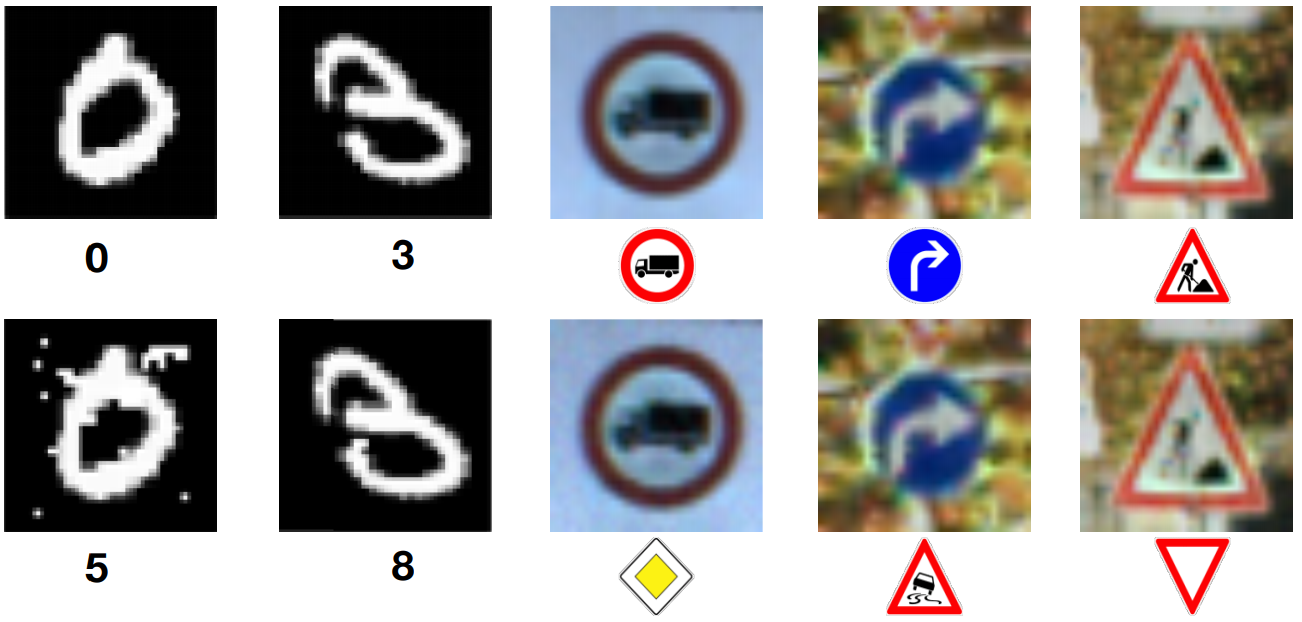
\includegraphics[width=11cm]{img/WrongPictures.png}
	\caption{The upper line of pictures shows the correctly recognized images (pictures had no adversarial information combined with original image). The bottom line of pictures shows captured pictures, combined with adversarial information, and what is recognized with the same algorithm \cite{blackBox1}}
	\label{fig:WrongPictures}    
\end{figure}

Attacks, introduced in \cite{blackBox1} are effective, but it is much harder to make it a real life rather than in the laboratory. The advertiser usually does not have direct access to control what is coming as an input to a vision recognition algorithm. As well, usually there are a bunch of other pictures of the same place in different directions and angles, so different algorithms can compare the pictures of the same place in different situations. And the last thing which does not usually work in the real world is that adversarial images contain the same features in all image not separating traffic sign or background. \\
The difference of method proposed in \cite{signs} is based on changing the sign physically - to alter signs in the way that visual recognition algorithms would be not able to correctly recognize the sign. For that author came with some "sign damaging" techniques: "subtle fading, camouflage graffiti, and camouflage art". Figure ~\ref{fig:perturbedsigns} shows how perturbed signs, used in experiments, look like.

\begin{figure}[H]
	\centering  	
	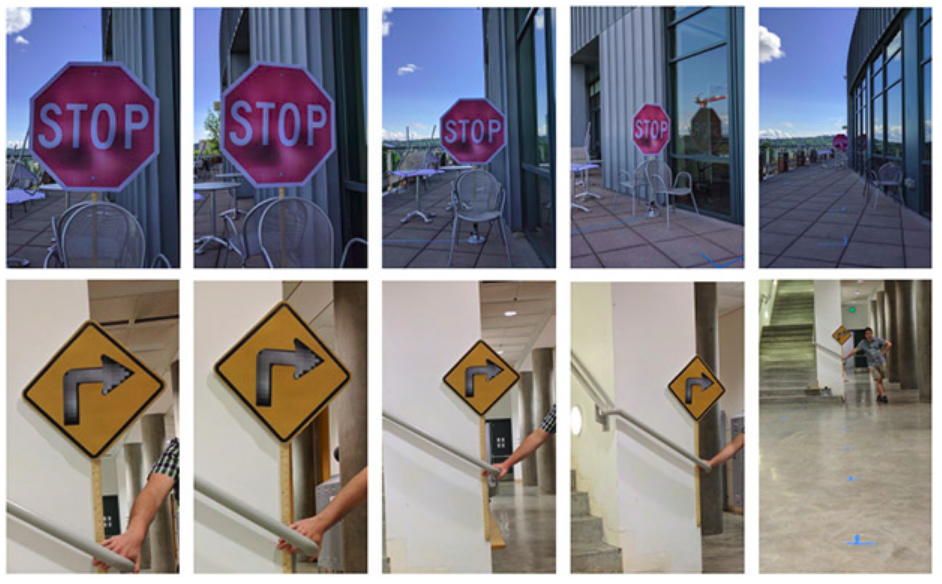
\includegraphics[width=11cm]{img/perturbedsigns.png}
	\caption{Small perturbations on signs resulted in misclassification of stop signs and think that it is speed limit 45 sign. The sign to turn right was recognized as a stop sign \cite{signs}}
	\label{fig:perturbedsigns}    
\end{figure}

There are different and easier ways to "damage" signs to mess up with visual recognition algorithms. It is possible to add some stickers or graffiti on signs as in  Figure ~\ref{fig:stickersigns}.

\begin{figure}[H]
	\centering  	
	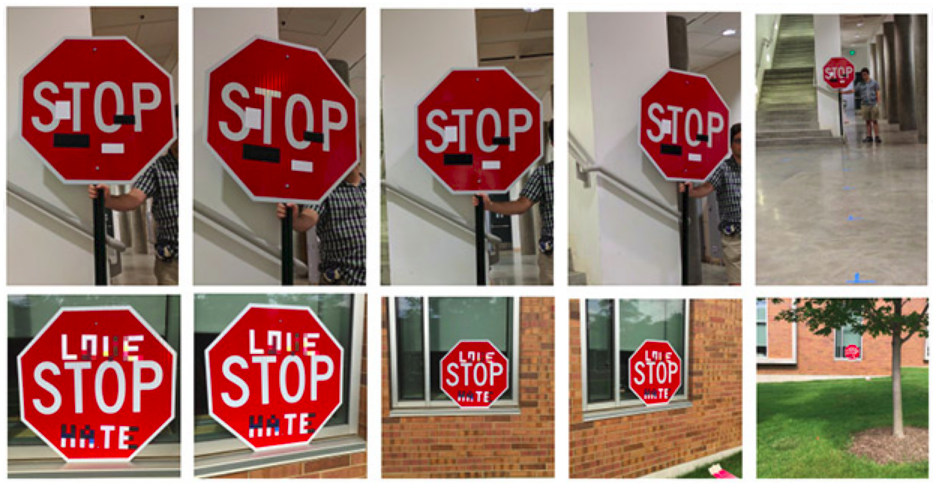
\includegraphics[width=11cm]{img/stickerSign.png}
	\caption{Camouflage graffiti and art stickers caused visual recognition algorithms to recognize stop sign as speed limit 45 \cite{signs}}
	\label{fig:stickersigns}    
\end{figure}

Due to being smaller, stickers have a visibly smaller zone, their created perturbations have a more significant impact on sign recognition but less visible by the human eye, and it worked as well. According to the authors of \cite{signs}: \textit{"The Stop sign is misclassified into our target class of Speed Limit $45$ in $100$\% of the images taken according to our evaluation methodology. For the Right Turn sign… Our attack reports a $100$\% success rate for misclassification with $66.67$\% of the images classified as a Stop sign and $33.7$\% of the images classified as an Added Lane sign. [The camouflage graffiti] attack succeeds in causing $73.33$\% of the images to be misclassified. In [the camouflage abstract art attack], we achieve a $100$\% misclassification rate into our target class"}. \\
Authors of \cite{signs} for algorithm training used publicaly available labeled data set. They assumed that the attacker won't be possible to play around with training data, but he can send images into an algorithm and see what results are coming out, to be able to see how algorithm recognize signs. And at the end authors took the "normal" image of the sign which is going to be attacked, gave it to the algorithm and received an adversarial image for result. It is probably a good assumption to make those classifiers which are used for autonomous vehicles have more sophisticated and robust than those which were used by authors. And it would be naive to think that hackers won't ever figure it out how to walk around even the most sophisticated and robust classifier ever. Probably the best defense against these attacks would be to use a multi-modal system for road sign detection as they are using it for obstacle detections - it is not very wise to trust only one sensor for these crucial tasks \cite{signs2}.

\subsection{Privacy Issues}

While autonomous cars might sound very convenient and create new forms of accessibility, we do need to remember that most of this comfort comes at a very big cost of privacy. To be able to ensure safety rides and all comfortability most of the people are expecting autonomous cars has a number of various sensors, which are proceeding a lot of data. Basic sensors of the car is visualized in Figure~\ref{fig:Sensors}. \\ 

\begin{figure}[H]
	\centering  	
	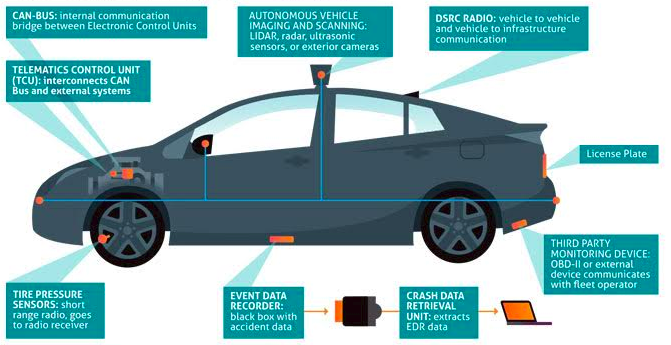
\includegraphics[width=11cm]{img/Sensors1.png}
	\caption{The Basic Data-Generating Devices and Flows in Autonomous Cars \cite{PicPrivacy}}
	\label{fig:Sensors}    
\end{figure}

Article \cite{ThreatenPrivacy} provides a very clear scenario of how "Automated vehicles will learn everything about you—and influence your behavior in ways you might not even realize". Most of the people in the morning go at work, so considering the time of the day, when an owner of the car gets into it, an autonomous vehicle will ask (or suggest) about driving at work first. Later, during the ride to work, car's owner want to take a coffee and car can suggest the coffee store or inform about sales and other offers which are happening in the stores which are on the route to work. On first sight, it might look awesome, but on the other hand to make these suggestions car needs to have some sensitive information about car's owner life and habits, as well as potentially be influenced to announce sponsored content. When a car makes an offer to go to work, it knows that at this particular time, the car is used to go to work. When a car gives you information about sales and coffee place, the order of offers coming out is based on how much business paid to advertise this offer (more expensive advertisement is, faster it is announced). Even though a lot of people can not see any problems with it, however, it can hide two big problems. First, car for obvious reasons always retains information where the car is and this can be very valuable knowledge for attackers/hacker. By knowing the place where and when the owner of the car is working, the attacker can make an assumption about the financial status of the car owner and knowing the time he is not at home, an attacker can easily break into his house and rob it. Additionally, during the robbery, an attacker can still track the car location and whenever car starts to move from current location, it can indicate that owner os potentially coming back to home and it is about time to leave. The second problem is that accepting the first location car suggested could give the car's owner personal data to marketers for highly specific marketing purposes without him/her even knowing this. \\
To consider these aspects is very important while thinking about the adaptation of autonomous cars, however, all legislation on autonomous cars so far are very vague when it is related to the aspect of privacy. So far only plan to keep the car owner informed how and where his data will be used is defined \cite{ThreatenPrivacyII}. This is a start, but still privacy issue not even close to being clear. A lot of people agree that it is crucial to regulate at least "minimum acceptable level of security" when it comes to data from autonomous cars, as there are minimum safety standards for the cars nowadays. We already have a very high number of issues for privacy which is related to the usage of smart technologies and it would be wise to think that the number of issues only grow with autonomous cars. Laws for privacy as always difficult to define, however, these questions are crucial for a secure transition to the safe world with autonomous cars. \\
Personal privacy is not the one concern which needs to be addressed. The case in 2016 when FBI was trying to force Apple to give access to personal iPhone of person who was suspected to be a shooter in San Bernardino attacks \cite{ThreatenPrivacyIII}, raised a legal issue: in which precedent manufacturer can (or need) to give personal user data to law enforcement. In the case, mentioned in \cite{ThreatenPrivacyIII}, the phone was an Apple product, but the data stored in the phone was the individual property of the phone owner. Could the law enforcement/government force the manufacturer of the autonomous vehicle to decrypt the personal data and give all information where someone was and where potentially could go? Again, on the first sight, it can look very innocent for cars' manufacturer to reveal the data of "dangerous" person, but this as well could affect the general consumer. When the manufacturer create a "back doors" which can give access to data of the user, just for "in case" scenario, these "doors" can be used not only by the manufacturer, it can be used by a malicious hacker to access a data and gain an important information which could be used to harm innocent autonomous car owner. In theory, to be able to protect consumers data, a manufacturer should ensure a security level of a device/car that even they could not get access to it in any cases: yes, this can save some criminals from being caught easier, but it would protect the vast majority of the people, who has a legal right to want that their information would be protected \cite{ThreatenPrivacyIV}. \\
Data and personal privacy is always a big concern when it comes to any type of technology which uses data, however, autonomous cars will have an "access" to people personal lives starting with car's location to environ them around it. With roads full of sponsored cars there will be no way that someplace and information about it will not be recorded, processed and stored. Due to that ensure safe storage for data is one of the most crucial tasks \cite{ThreatenPrivacyIV}.